\documentclass[12pt]{article}
\usepackage[brazil]{babel} % idioma PT-BR
\usepackage{indentfirst} % esse pacote aplica a indentação
%\setlength{\parindent}{1cm} % este comando altera a indentação do parágrafo
%\setlength{\parskip}{.5cm} % este comando altera o espaço entre parágrafos
\usepackage{setspace} % esse pacote altera o espaçamento entre linhas
\usepackage[a4paper, left=3cm, right=2cm, top=3cm, bottom=2cm]{geometry} % este pacote altera a margem do documento
\usepackage[usenames, dvipsnames]{xcolor} % modifica as cores
\usepackage{graphicx} % este pacote permite adicionar figuras
\usepackage{float} % força o posicionamento da figura
\usepackage{amsmath} % Modo matemático
\usepackage{url}

\begin{document}
    \begin{figure}
        \centering
        
\includegraphics[width=0.35\linewidth]{Figuras/ufsj-logo-2018}
        \\\setlength{\parskip}{1cm}
        \textbf{UNIVERSIDADE FEDERAL DE SÃO JOÃO DEL-REI}
        \label{fig:ufsj-logo-2018}
    \end{figure}

    \title{ 

        Algoritmo e estrutura de dados III 
		
        \vspace{5cm} % adiciona espaço entre parágrafos
		    \textbf{HIPERCAMPOS}
		\vspace{5cm} % adiciona espaço entre parágrafos
	}
	\setstretch{1.5} % define o tamanho do espaçamento de linhas 
    \author{Prof.: Dr. Leonardo Rocha \\ Gustavo Henriques \\ Matheus N Silva}
    \date{São João del-Rei, 11 de abril de 2023}
    \maketitle
    \thispagestyle{empty} % remove numeração da pagina
    \newpage
    
    \setcounter{page}{1} % Inicia a ordem de numeração das paginas
    \pagenumbering{Roman} % Estilo de numeração Romana
    \tableofcontents % Cria sumário
    \newpage
    
    \setcounter{page}{1} % Inicia a ordem de numeração das paginas
    \pagenumbering{arabic} % Estilo de numeração Arábica
    \section{INTRODUÇÃO} % Titulo da secção
        \subsection{Proposta}
            Foi proposto como primeiro trabalho prático da disciplina de Algoritmo e
            Estrutura de Dados III a implementação de uma aplicação onde, a partir de 
            uma entrada de N pontos (sendo que dois desses pontos são ancoras), 
            conseguisse computar o número máximo de pontos que seja possível conectar 
            através de segmentos de reta, sendo que sua intersecção só exista nos pontos
            ancoras, ou seja, sem que esses segmentos se intersectem no caminho.
            
            
        \subsection{Objetivo}
            Após a implementação da aplicação o objetivo principal torna a ser a obtenção de 
            dados referente à sua execução, tanto dados finais, tais como resultados corretos, 
            como seu desempenho durante a mesma.

            Para chegarmos à esses dados a aplicação foi testada inúmeras vezes com vários
            parâmetros distintos de entrada 
            
            Através deste trabalho foi testado e aprimorado os conhecimentos
            até aqui adquiridos durante o curso.
        \subsection{Execução}
            Para compilar e executar a aplicação deve-se abrir o terminal na pasta 
            do arquivo (ou navegar até a pasta do arquivo) e digitar os seguintes comandos:
            \begin{itemize}
                \item Compilar: 
                \begin{itemize}
                    \item[\$] make
                \end{itemize}
                \item Executar: 
                \begin{itemize}
                    \item[\$] ./main -i "nome\underline{ }arquivo\underline{ }entrada".txt -o "nome\underline{ }arquivo\underline{ }saida".txt
                \end{itemize}
                \item Teste:
                \begin{itemize}
                    \item[\$] ./auto.sh
                \end{itemize}
            \end{itemize}
    \newpage
    \section{IMPLEMENTAÇÃO}
        Este capitulo apresenta de forma breve algumas explicações e comentários
        a respeito da implementação dos algoritmos utilizados para a resolução da proposta.
        \subsection{Main}
            A main apresenta as chamadas dos métodos principais da aplicação. É nela também
            que estão declaradas algumas variáveis (obrigatórias) utilizadas.\\\\
            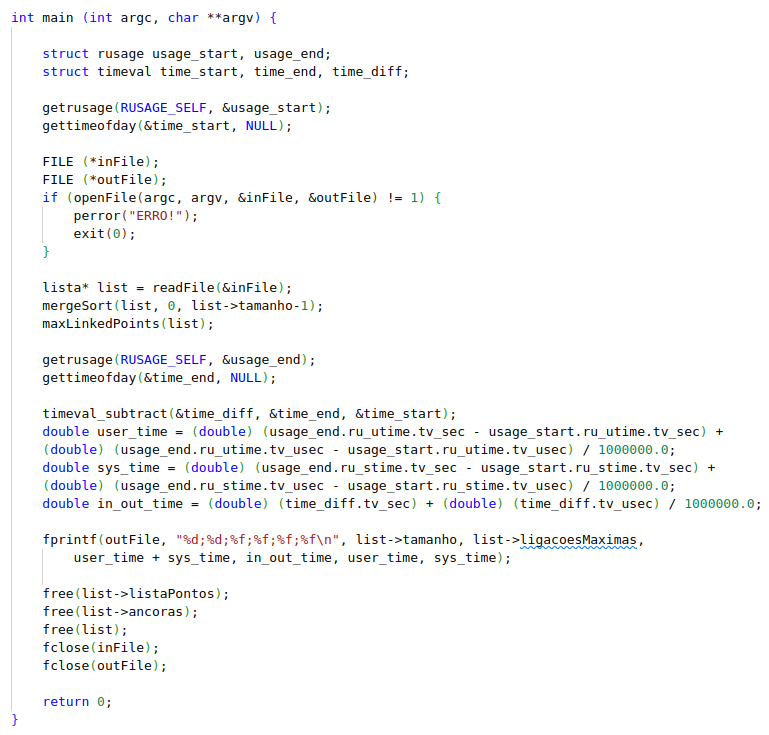
\includegraphics[width=1.0\linewidth]{Figuras/1.1.png}\\
            Nota-se que estão declaradas variáveis de estruturas Rusage e Timeval onde serão
            armazenadas o tempo de programa e o tempo de relógio respectivamente.
            Após a inicialização dessas variáveis são abertos os arquivos de entrada e saida
            passados via terminal, sendo acionado o método de leitura do arquivo de entrada
            preenchendo assim à estrutura de armazenamento dos dados. Na sequencia é realizado
            a ordenação dessa estrutura para que possa ocorrer o calculo da quantidade maxima
            de pontos que podem ser interligados a partir das ancoras sem ocorrer intersecção 
            entre eles.      
        \subsection{Cálculo de intersecção}
            O método maxLinkedPoint é o próximo a ser chamado pelo main. Ele recebe uma lista com
            os pontos a serem interligados e verifica através do método isInside se os pontos estão 
            abaixo da intersecção superior.\\\\
            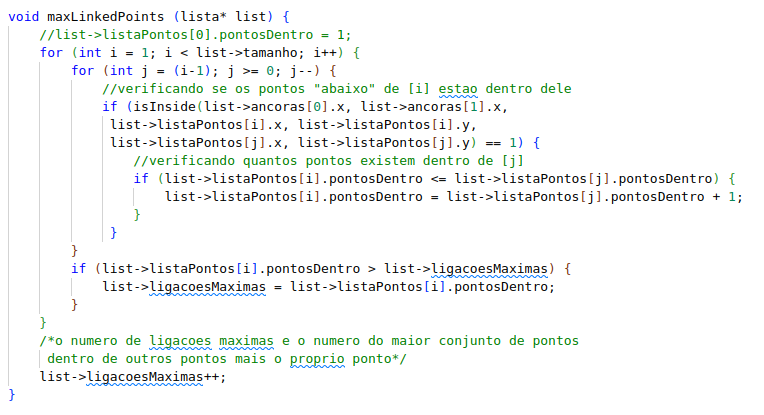
\includegraphics[width=1.0\linewidth]{Figuras/2.png}\\
            Observando o algoritmo acima é possivel notar que após calcular a quantidade maxima
            de ligações possíveis é necessário adicionar mais uma ligação, que seria a intersecção 
            superior.\\\\
            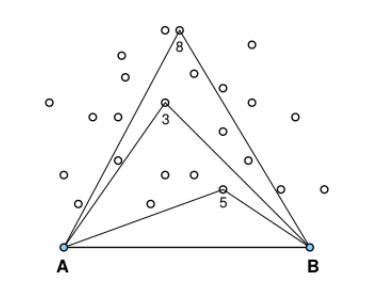
\includegraphics[width=0.35\linewidth]{Figuras/5.png}
            \textit{Obs.: No exemplo ao lado a intersecção superior é apresentada pelos segmentos de reta A8 e B8.}\\
            
            O método isInside recebe as duas ancoras e as coordenadas x e y de cada ponto à ser verificado. \\\\
            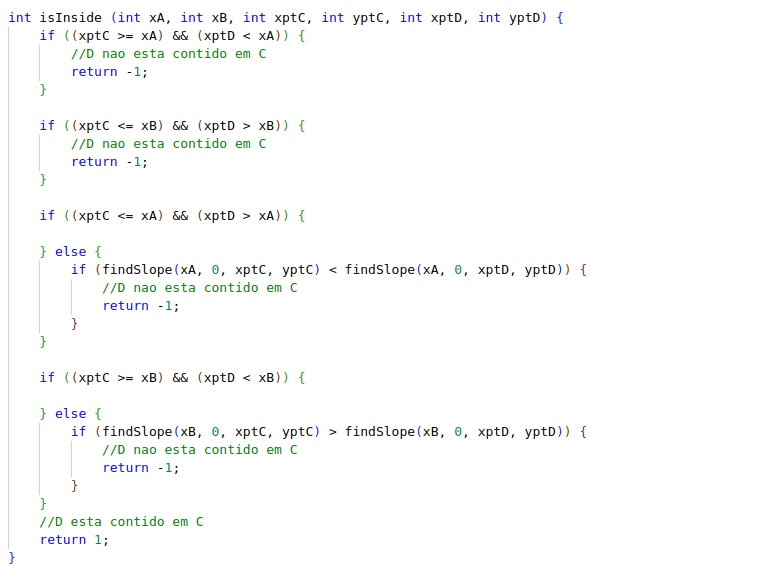
\includegraphics[width=1.0\linewidth]{Figuras/4.png}\\
            Para que ocorra a verificação de forma correta é necessário que se calcule o coeficiente angular da reta
            tarefa essa designada ao método findSlope\\\\
            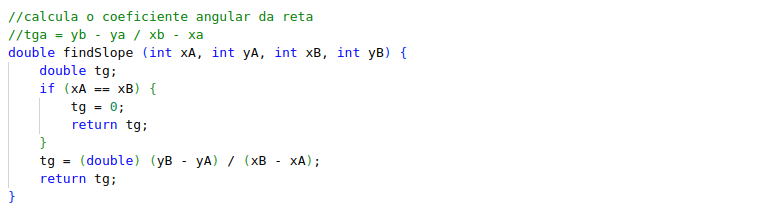
\includegraphics[width=1.0\linewidth]{Figuras/3.png}\\

    \newpage
    \section{COMPLEXIDADE}
        Para calcularmos a complexidade do algoritmo desenvolvido iremos utilizar apenas o 
        calculo de intersecção, tendo em vista que de todos os métodos, ele é o mais custoso. 
       
        Devemos então observar o algoritmo novamente.\\\\
        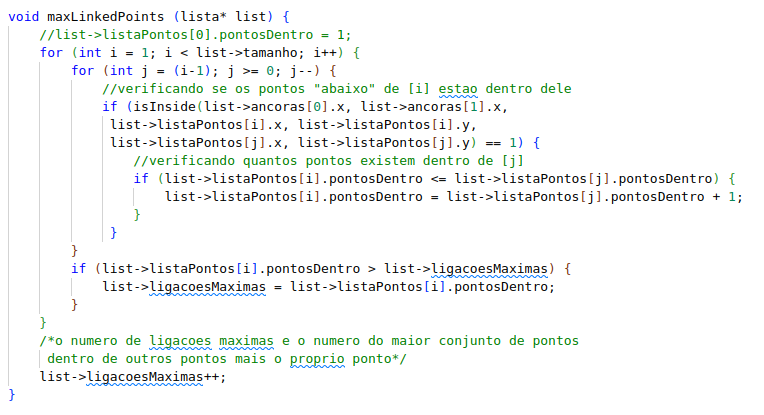
\includegraphics[width=1.0\linewidth]{Figuras/2.png}\\
        Podemos notar que o algoritmo possui um laço \textbf{for} aninhado dentro de outro laço 
        \textbf{for}, instintivamente ja falaríamos \textbf{O(n²)} mas porque a complexidade dele é
        essa?
        Observando cada parte do algoritmo notamos que o laço interno é executado n vezes, ja o laço
        externo é executado n-1 vezes. Então para descobrirmos a complexidade precisamos utilizar um 
        somatório:
        \[\sum_{1}^{n-1}(n-1) = \frac{n(n-1)}{2} = \frac{n^2-n}{2}\]
        
        \textit{Obs.: Ignoramos o custo das atribuições, incrementações e comparações pois em todos 
        os casos o custo de tais operações é sempre constante.}\\
        
        Como sempre tomamos o termo mais "custoso" da função como base, temos que a aplicação é O(n²). 
        Após esse calculo ainda seria necessário adicionar o custo da ordenação, mas como o merge sort é, 
        notoriamente, O(n log n), podemos "ignorar", já que a ordem do método principal o domina 
        assintoticamente.

    \newpage
    \section{AVALIAÇÃO DE RESULTADOS}
        Foram realizados testes com mais de cinquenta entradas diferentes, utilizando um shellscript para tal,
        sendo o mesmo executado algumas vezes para a obtenção de um maior número de dados para comparação.
        Os resultados obtidos após essa bateria de testes estão representados na tabela abaixo:
        \begin{table}[h!]
            \centering
            \begin{tabular}{|l|l|l|l|}
                \hline
                Entrada & Saida & Tempo (Sys + User) & Tempo Relógio \\ \hline

                7590 & 156 & 0.567s & 0.566s \\ \hline
                7666 & 31 & 0.446s & 0.445s \\ \hline
                2002 & 62 & 0.040s & 0.040s \\ \hline
                7897 & 95 & 0.567s & 0.566s \\ \hline
                6233 & 72 & 0.373s & 0.373s \\ \hline
                5500 & 102 & 0.302s & 0.308s \\ \hline
                3034 & 59 & 0.080s & 0.079s \\ \hline
                5781 & 100 & 0.298s & 0.300s \\ \hline
                5128 & 64 & 0.221s & 0.220s \\ \hline
                6629 & 149 & 0.441s & 0.441s \\ \hline
                282 & 18 & 0.006s& 0.004s \\ \hline
                353 & 24 & 0.004s & 0.003s \\ \hline
                5421 & 36 & 0.272s & 0.271s \\ \hline
                662 & 13 & 0.008s & 0.007s \\ \hline
                9448 & 128 & 0.833s & 0.833s \\ \hline
                4433 & 115 & 0.196s & 0.195s \\ \hline
                2407 & 28 & 0.047s & 0.046s \\ \hline
                3920 & 16 & 0.134s & 0.134s \\ \hline
                2912 & 76 & 0.113s & 0.112s \\ \hline
                4301 & 79 & 0.176s & 0.177s \\ \hline
            \end{tabular}
        \end{table}\\
        \textit{Obs.: Nessa tabela são apresentados apenas 20 resultados obtidos tendo em visa
        que não há necessidade de se avaliar todos os testes efetuados.\\
        Obs².: As configurações de hardware utilizados para os testes são as seguintes:\\ 
        CPU: Intel i7-10750H, RAM: 16gb - 2933mhz, SSD: WD blue 250gb - 2400Mb/s, \\SO: Ubuntu 22.04.2 lts,
        COMPILADOR: GCC v11.3.0.}\\

        Podemos notar que o tempo de relógio não difere tanto quando comparado ao tempo de sistema 
        somado ao de usuário. O resultado final de ambos esta diretamente relacionado ao tamanho de entrada fornecida.
        
    \newpage
    \section{CONCLUSÃO}
        Para realização desse trabalho prático foram necessárias algumas, várias, horas de pesquisas,
        alem de teste e mais testes, muitas frustrações com métodos que não funcionavam do jeito que queríamos
        mas ao fim de tudo a aplicação saiu como desejamos.

        Esse trabalho prático exigiu muito mas também agregou muito conhecimento à todos os membros do grupo.
	\newpage
    \nocite{Cormen2012}
    \nocite{Backes2012}
	\nocite{Backes2016}
    \nocite{GNU}

	\addcontentsline{toc}{section}{REFERÊNCIAS}
	\bibliographystyle{apalike} % Estilo da bibliografia
	\bibliography{bibliografia} % Adiciona as referencias
\end{document}